\section{The \texttt{v4.0} simulations} \label{sec:baseline4_0}

The \baseline{4.0} simulation embodies the recommendations of the SCOC presented in this document. 

There are slightly more than 2 million visits in \baseline{4.0}, split between different regions on the sky and different modes of observing. The Wide Fast Deep area (WFD) consists of a low dust extinction area (\mbox{$\approx$17,800} square degrees) and an additional \mbox{$\approx$2,000} square degrees within the Galactic Plane and the LMC/SMC areas. About 138,000 visits (6.8\% of the total) are spent in the five Deep Drilling Fields (DDFs), with the COSMOS field receiving an additional \mbox{$\approx$20,000} visits in order to reach the 10-year Deep Drilling Field depth within the first three years (\citetalias{PSTN-055} \S2.6.1). The North Ecliptic Spur (NES), South Celestial Pole (SCP) and the remainder of the galactic plane (``dusty plane'') round out the footprint of the survey. Within the Galactic Plane WFD region, some visits (\mbox{$\approx$1,600}) are shifted to provide additional coverage at the location of the Roman Bulge Time Domain Survey (\autoref{sec:subG:footprint}). 

\begin{figure}
  \centering
    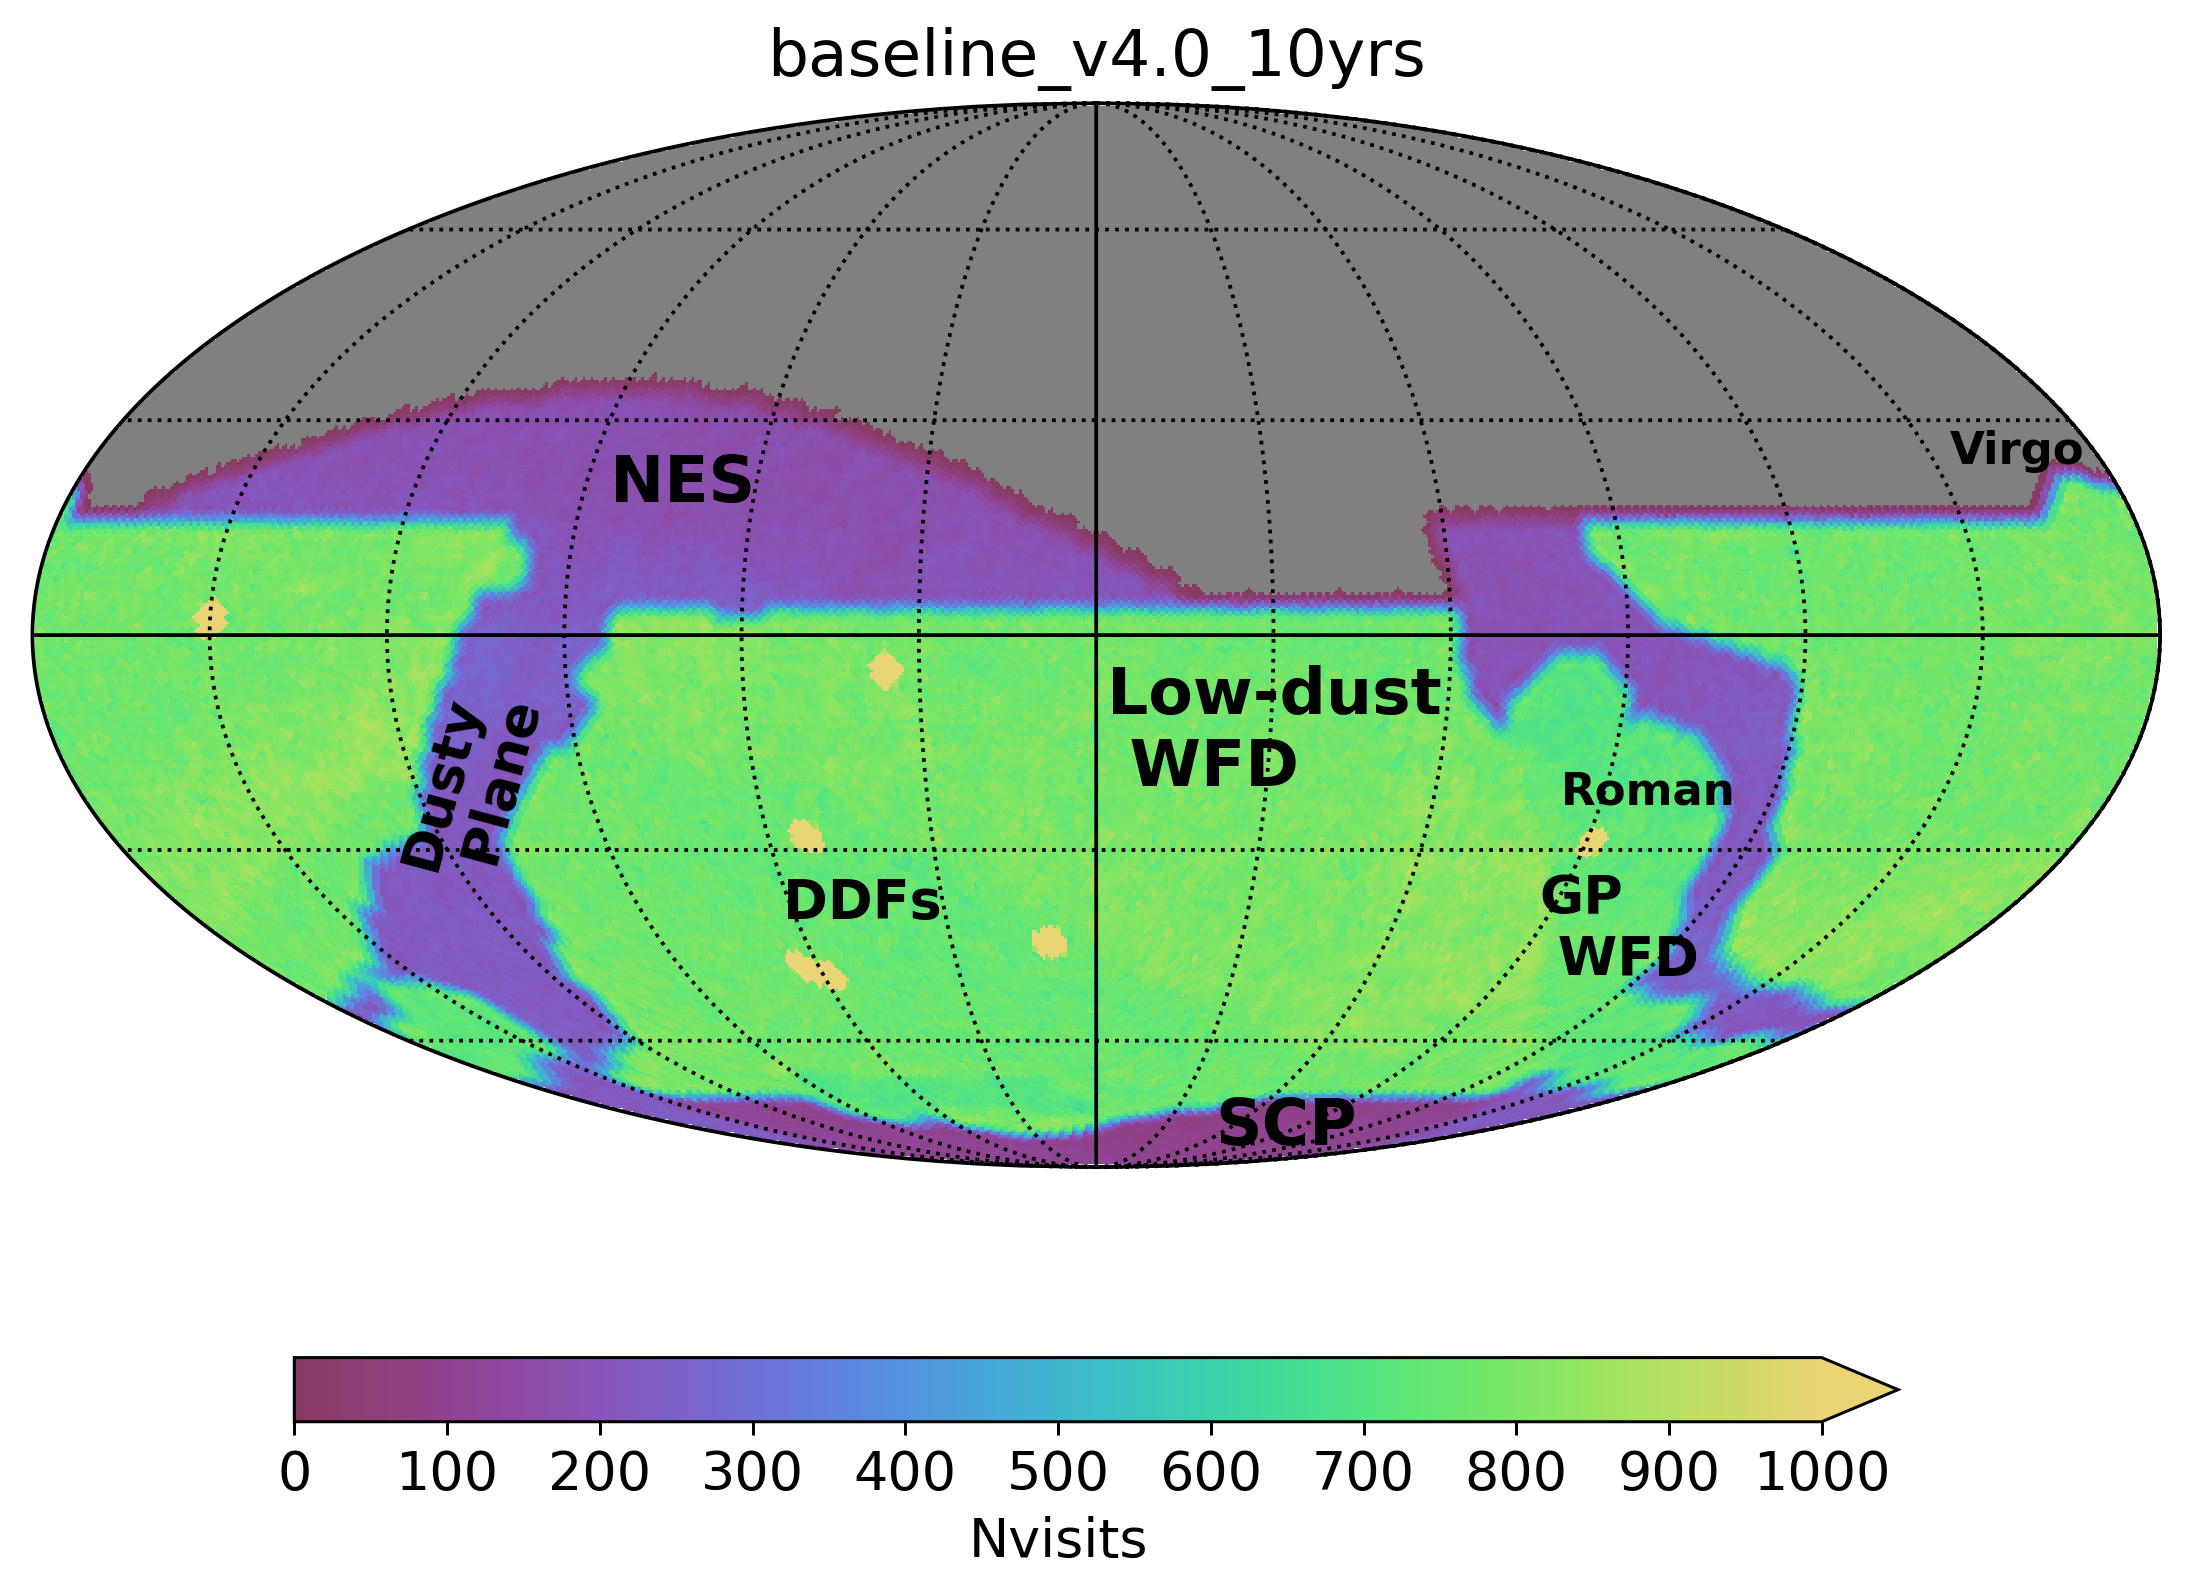
\includegraphics[width=0.7\linewidth]{figures/baseline_v4_0_10yrs_nvisits.png}
    \caption{The \baseline{4.0} footprint, with labels indicating different survey regions.}
    \label{fig:footprint_v4}
\end{figure}

In all of these regions on the sky, visits within a night are attempted in pairs, with each first visit to a pointing paired with a return visit typically 33 minutes later in a different filter. This provides the opportunity to measure colors for transient or variable objects. Visits are paired as follows: $u+g$ or $u+r$, $g+u$ or $g+r$, $r+u$ or $r+i$, $i+r$ or $i+z$, $z+i$ or $z+y$, $y+z$ or $y+y$ (\citetalias{PSTN-053} \S3).  During twilight, the interval between these pairs may be shorter or visits may be scheduled as singles instead of paired. Approximately 4\% of all visits are part of a triplet of visits, instead of just a pair. In these cases, the first pair is followed several hours later by a third visit, in a filter matching the earlier pair. This enables probing short timescale variability, although at the cost of increased slew time and obtaining observations at higher airmass (\citetalias{PSTN-055} \S2.4). 

Within the low-dust WFD footprint, a rolling cadence is followed. This rolling cadence distributes visits unevenly across seasons; in some seasons, a portion of the footprint will receive more than the typical number of visits while, in other seasons, the same portion of the footprint will receive fewer than the typical number of visits. The exact details of how many more or less visits are received in alternating seasons depends on the `strength' of the rolling cadence as well as the typically number of visits in a season and the minimum number of visits in any season needed in order to continue creating templates for difference imaging (\citetalias{PSTN-055} \S2.5). In \baseline{4.0}, the high and low seasons correspond to 125 and 25 visits, with a typical season of 75 visits. The low-dust WFD region is split into four declination bands, two of which are active in a high season, while two are in a low season at any point when rolling cadence is active at that point in the sky (\citetalias{PSTN-055} \S2.5). A `cycle' of rolling consists of two seasons, so that both a high and low cadence season can occur. In \baseline{4.0}, there are three cycles of rolling cadence at each point on the sky, with a uniform (non-rolling) season in between each of these seasons. This `Uniform Rolling' cadence provides the opportunity for higher uniformity at intermediate data releases in year 4 and 7 (\autoref{sec:rolling}). 

The filter balance within different areas of the footprint varies. Per pointing, the low-dust WFD obtains a median of 54 visits in $u$ band, 66 visits in $g$ band, 174 in $r$ and 176 in $i$ bands, and 158 in $z$ and 155 in $y$ bands (\autoref{sec:filterbalance}). The Galactic Plane WFD region tilts the balance toward fewer $u$ and $y$ band visits and more $g$ band (\autoref{sec:subG:filterbalance}), while the LMC/SMC region gets fewer $z$ and $y$ band visits to obtain more $u$ and $g$ band visits (\autoref{sec:subG:specialregions}). The dusty plane region focuses on $g$, $r$, $i$, and $z$, with fewer visits in $u$ and $y$. The NES only obtains visits in $g$, $r$, $i$, and $z$ band as these are the most useful for Solar System objects (\citetalias{PSTN-053} \S3). The SCP region uses its fewer visits per pointing with a higher fraction of $g$, $r$ and $i$ band visits.

The Near-Sun Twilight microsurvey is implemented in Y1 because it is at risk of interference by satellite constellations in later years (\citetalias{PSTN-055} \S2.7.2). It runs every fourth night at both evening and morning twilight, obtaining quads of short (15~seconds) visits in $g$, $r$, $i$ and $z$ bands at high airmass towards the Sun. These low solar elongation visits permit detection of interior-to-earth asteroids. %Additional microsurveys will be considered by the SCOC, to be added as survey observing time permits.

Target of Opportunity observations are simulated in \baseline{4.0}, matching the 2024 Rubin ToO Workshop outcomes and SCOC recommendations (\autoref{sec:ToO}). The bulk of these ToO visits correspond to followup of GW events during the estimated dates of LKV O5. Additional ToO visits are dedicated to following Solar System and neutrino triggers. The fraction of on-sky time spent in ToOs in \baseline{4.0} is between 3 and 4\%. 

The simulations provided in \texttt{v4.0} include
\begin{itemize}
    \item \texttt{baseline\_v4.0\_10yrs} - the baseline simulation as described above
    \item \texttt{four\_cycle\_v4.0\_10yrs} - a simulation similar to the one described above, except using four cycles of rolling cadence in the low-dust WFD instead of three cycles interspersed with uniform seasons. 
    \item \texttt{one\_snap\_v4.0\_10yrs} - a simulation similar to the baseline, but using single exposures for all visits instead of two exposures per visit in $g$, $r$, $i$, $z$ and $y$ bands. %This improves the duty cycle of observing and increases the efficiency of the survey.
\end{itemize}
